\section{Visual Perception}

\subsection{Field of View}

How much of the field of view is obstructed, depends on the design and distance of the suit's face shield (see figure below).

GRAPHIC FOV, wide vs narrow face shield, long vs short distance
- wider/less distance to face = bigger view angle

\subsection{Peripheral Vision}

\begin{figure}[hbt]
    \centering
    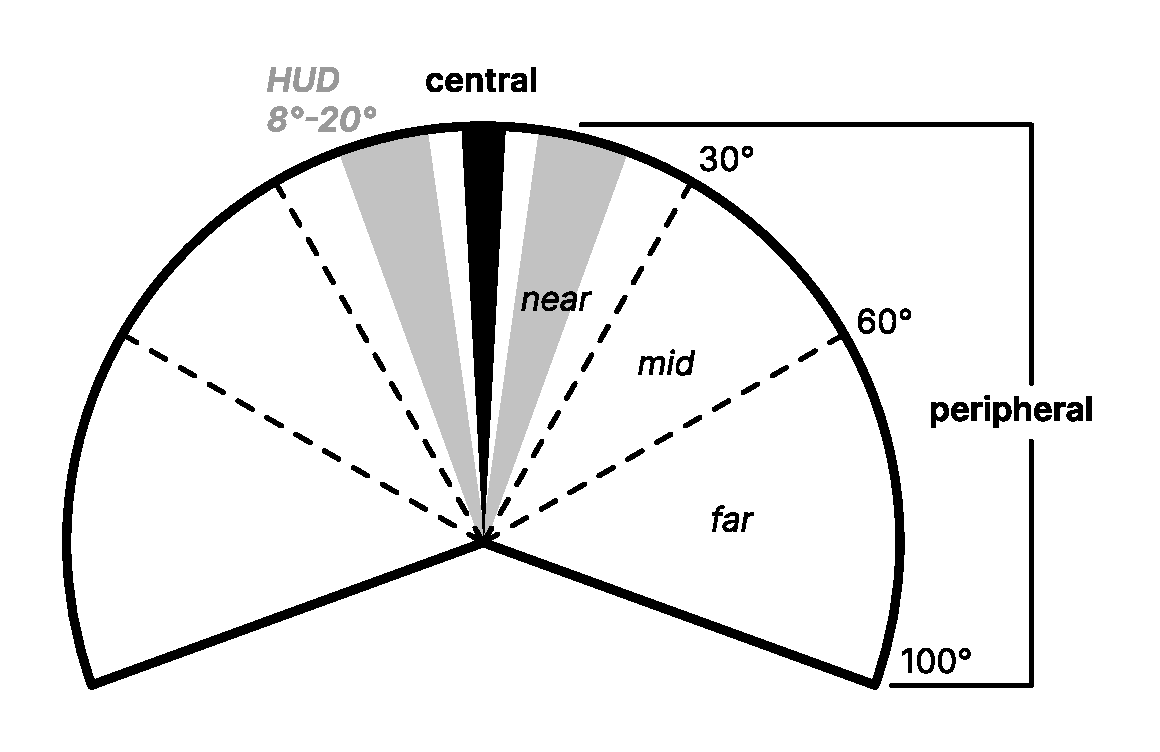
\includegraphics[width=0.5\textwidth]{assets/FOV.eps}
    \caption{Simplified field of view}
    \label{fig:FOV}
\end{figure}

The peripheral vision is especially important to recognize hazards quickly, and should not be obstructed [\cite{}].

\textcite{rosenholtzCapabilitiesLimitationsPeripheral2016} suggests that crowding is the biggest issue when it comes to parsing information.

better sight in low light bc of rods (more populated in peripheral)

focus on (pre-)peripheral as limit/"frame" for projected UI

---

EYE STRAIN with light-emitting displays
does that get worse if the display is closer to the eye?
is eye strain linked to earlier exhaustion/other relevant negative effects?

trade-offs: low contrast vs visibility?

is there a brightness threshold for distraction?

---

how does acute stress/panic affect vision? what about physical emergencies, like dizziness? fov narrower? vision loss? blur?
assume that color is still recognizable

---

recognition of contrasts in general better? (e.g. if everything moves, a detail that doesn't will also be found)

\subsection{Perceptual Psychology}

reaction to color + movement

blinking bad? frequency?

---

speed of comprehending/parsing information

---

- mitigating autopilot mode for routine tasks

inattentional blindness